\documentclass{automatisme}

\begin{document}

\begin{frame}
	Les points ci-dessous sont-ils alignés ?

	\begin{center}
		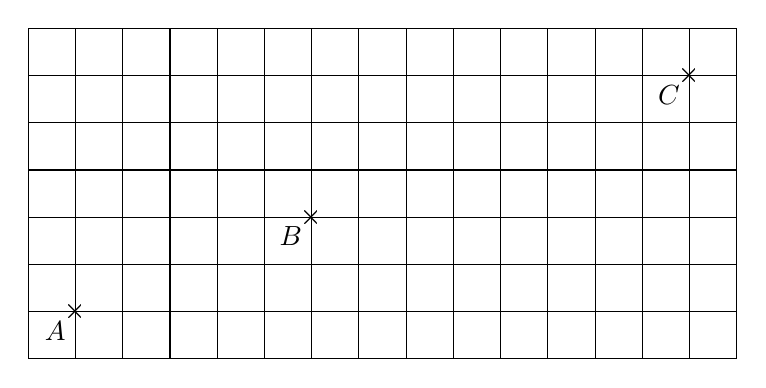
\begin{tikzpicture}[scale=0.6]
			\coordinate (A) at (0,0);
			\coordinate (B) at (5,2);
			\coordinate (C) at (13,5);

			\foreach \p in {A,B,C} {
				\node at (\p) {×};
				\node[below left] at (\p) {$\p$};
			}

			\draw<2> (-1,-1) grid (14,6);
		\end{tikzpicture}
	\end{center}
\end{frame}

\end{document}